\section{Evaluation}

We evaluate the implemented algorithm on doth regular and context-free path queryes in order to demonstrate applicability of the proposed solution.
Namely, goals of the evaluation are following.
\begin{enumerate}
	\item Investigate practical applicability of RPQ evaluation by the proposed algorithm.
	\item Compare Azimov's algorithm for reachability CFPQ and the proposed algorithm.
	\item Investigate practical applicability of paths extraction algorithm for both regular and context-free queries.
\end{enumerate}

For evaluation, we use a PC with Ubuntu 18.04 installed.
It has Intel core i7-6700 CPU, 3.4GHz, and DDR4 64Gb RAM.

\subsection{RPQ Evaluation}

In oder to investigate applicability of the proposed algorithm for RPQ over real-world graphs we collect a set of real-world and synthetic graphs and evaluate queries generated by using the most popular templates for RPQs.

\subsubsection{Dataset}

Collected graphs are presented in table~\ref{tbl:graphs_for_rpq}.
The dataset consists of several parts.
The first one is a set of LUBM graphs with different number of vertices, generated by~\cite{!!!}.
Second one is a graphs from Uniprot database\footnote{}~\cite{!!!}: \textit{proteomes} and \textit{!!!}.
RDFs and from DBPedia.


\begin{table}
\begin{tabular}{|l|c|c|}
\hline
Graph & \#V & \#E \\
\hline
\hline 
LUBM100  & 300000 & 4000000 \\
LUBM300  & 3 & 4 \\
LUBM1M   & 3 & 4 \\
LUBM1.5M & 3 & 4 \\
LUBM1.9M & 3 & 4 \\
\hline
Uniprotkb & 3 & 4 \\
Proteomes & 3 & 4 \\
\hline
Geospecies & 3 & 4 \\
DBPedia & 3 & 4 \\
\hline
\end{tabular}
\caption{Graphs for RPQ evaluation}
\label{tbl:graphs_for_rpq}
\end{table}


Queries for evaluation was generated by using templates of the most popular RPQs which are collected from~
\cite{!!!} and~\cite{!!!}, and are presented in table~\ref{!!!}.
We generate 10 queries for each template and each graph using the most frequent relations from the given graph randomly.

\subsubsection{Results}

Results of evaluation

Index creation.

\begin{figure}
   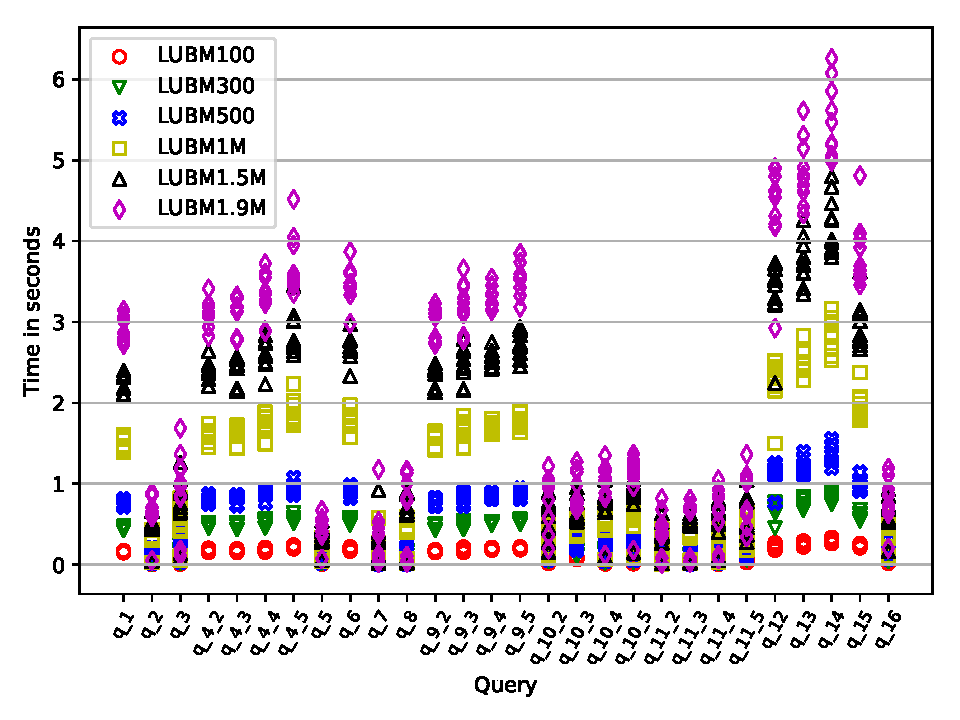
\includegraphics[width=0.48\textwidth]{data/LUBM_all.pdf}
   \caption{Reachability index creation time for LUNM series}
\end{figure}


\begin{figure}
   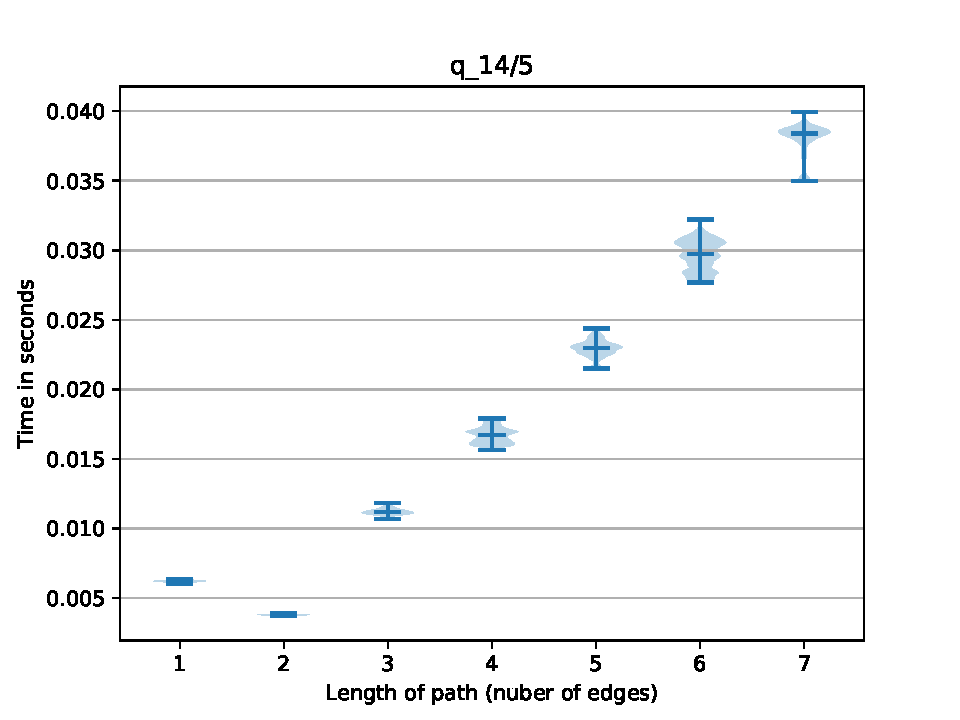
\includegraphics[width=0.48\textwidth]{data/res_graphics/q_14_5.pdf}
   \caption{Single path extraction}
\end{figure}

Paths extraction

\subsubsection{Conclusion}

\subsection{CFPQ Evaluation}

Comparison with matrix-based algorithm.

\subsubsection{Dataset}

Dataset for evaluation. 
It should be CFPQ\_Data\footnote{CFPQ\_Data is a dataset for CFPQ evaluation which contains both synthetic and real-world data and queries \url{https://github.com/JetBrains-Research/CFPQ\_Data}. Access date: 07.07.2020.}

Same-generation queries, memory aliases.

\subsubsection{Results}

Results of evaluation.

Index creation.

Paths extraction.

\subsubsection{Conclusion}
